\documentclass{standalone}
\usepackage{tikz}
\begin{document}
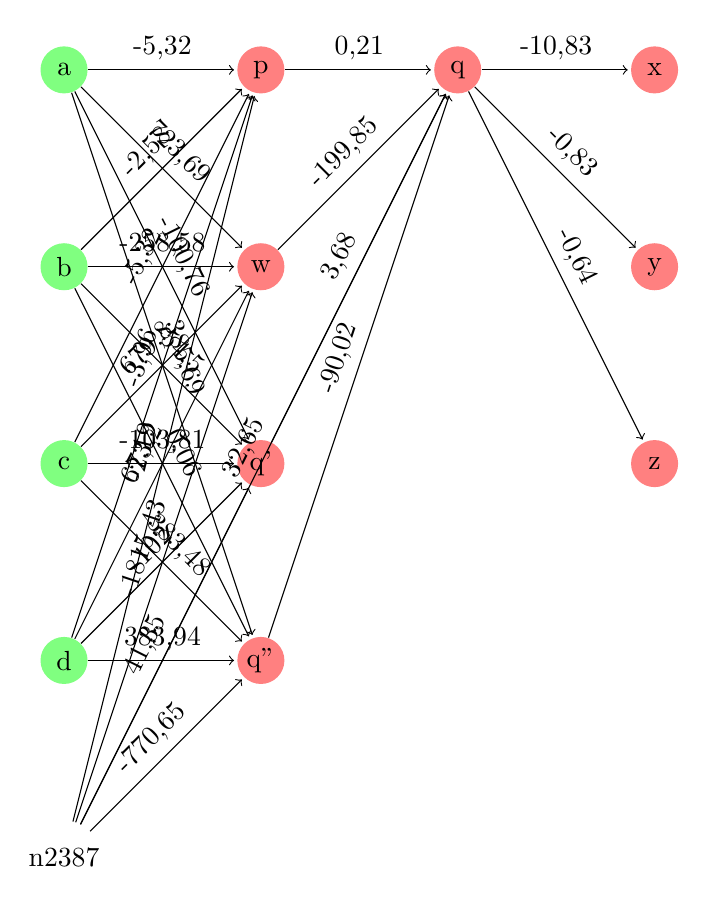
\begin{tikzpicture}[shorten >=1pt,->,draw=black!,node distance=2.5cm]
\tikzstyle{neuron}=[circle,fill=black!25,minimum size=17pt,inner sep=0pt]
\tikzstyle{constant}=[neuron, fill=white!50];
\tikzstyle{sigmoid}=[neuron, fill=red!50];
\tikzstyle{identity}=[neuron, fill=green!50];
\node [identity] (a) {a};
\node [identity,below of=a] (b) {b};
\node [identity,below of=b] (c) {c};
\node [identity,below of=c] (d) {d};
\node [constant,below of=d] (n2387) {n2387};
\node [sigmoid,right of=a] (p) {p};
\node [sigmoid,below of=p] (w) {w};
\node [sigmoid,below of=w] (q') {q'};
\node [sigmoid,below of=q'] (q'') {q''};
\node [sigmoid,right of=p] (q) {q};
\node [sigmoid,right of=q] (x) {x};
\node [sigmoid,below of=x] (y) {y};
\node [sigmoid,below of=y] (z) {z};
\path[every node/.style={sloped,anchor=south,auto=false}]
(p) edge node {0,21} (q)
(q') edge node {3,68} (q)
(w) edge node {-199,85} (q)
(a) edge node {-5,32} (p)
(a) edge node {-100,76} (q')
(a) edge node {723,69} (w)
(a) edge node {385,69} (q'')
(q) edge node {-0,83} (y)
(q) edge node {-10,83} (x)
(q) edge node {-0,64} (z)
(q'') edge node {-90,02} (q)
(c) edge node {-5,32} (p)
(c) edge node {-103,81} (q')
(c) edge node {679,8} (w)
(c) edge node {383,48} (q'')
(b) edge node {-258,58} (w)
(b) edge node {-2,58} (p)
(b) edge node {0,06} (q'')
(b) edge node {-54,5} (q')
(d) edge node {673,2} (w)
(d) edge node {-3,96} (p)
(d) edge node {383,94} (q'')
(d) edge node {-102} (q')
(n2387) edge node {-1815,43} (w)
(n2387) edge node {-2,19} (p)
(n2387) edge node {-770,65} (q'')
(n2387) edge node {41,35} (q')
(n2387) edge node {32,65} (q)
;\end{tikzpicture}
\end{document}